\documentclass[conference]{IEEEtran}
\usepackage{amsmath}
\usepackage{eurosym}
\usepackage{subcaption}
\usepackage[noadjust]{cite}
 \usepackage{graphicx}
\usepackage{algorithm, algorithmic}
\usepackage{xcolor}
\usepackage{listings}
\lstset{basicstyle=\ttfamily,
  showstringspaces=false,
  commentstyle=\color{red},
  keywordstyle=\color{blue}
}

\usepackage{mathtools}
\usepackage{longtable}
\usepackage{array}
\usepackage{multirow}
\newcolumntype{L}[1]{>{\raggedright\let\newline\\\arraybackslash\hspace{0pt}}m{#1}}
\newcolumntype{C}[1]{>{\centering\let\newline\\\arraybackslash\hspace{0pt}}m{#1}}
\newcolumntype{R}[1]{>{\raggedleft\let\newline\\\arraybackslash\hspace{0pt}}m{#1}}
\interdisplaylinepenalty=2500


\interdisplaylinepenalty=2500
\newcommand\Mark[1]{\textsuperscript{#1}}
\newcommand\fixit[1]{{\color{red}{\Large FIX:} #1}}
\begin{document}
%
% paper title
% Titles are generally capitalized except for words such as a, an, and, as,
% at, but, by, for, in, nor, of, on, or, the, to and up, which are usually
% not capitalized unless they are the first or last word of the title.
% Linebreaks \\ can be used within to get better formatting as desired.
% Do not put math or special symbols in the title.

\title{Implementation of ZNCC algorithm for disparity map computation using OpenCL}

\author{
    \IEEEauthorblockA{{\normalfont\large Aleksei~Tiulpin}\\Center for Machine Vision and Signal Analysis\\University of Oulu}
    \and
    \IEEEauthorblockA{{\normalfont\large Iaroslav~Melekhov}\\Department of Computer Science\\ Aalto University}
}


\maketitle


\begin{abstract}
In this report we describe an implementation of zero mean cross-correlation algorithm for stereo correspondence search. In particular, we show the accelerated implementation of the algorithm using OpenCL v.1.2 standard. The performance gain which we managed to achieve with the accelerated version of the algorithm is around 100 times.
\end{abstract}


\section{Introduction}
Estimation of a disparity map of an image sequence plays important role in such large areas of computer vision as multi-view image generation \cite{}, 3D reconstruction from stereo image pairs \cite{} and object recognition\cite{}. Obtaining a precise and accurate depth map is the ultimate goal in these applications.

By the definition, binoclular disparity is positional difference between the two retinal projections of a given point in space. This positional difference results from the fact that the two eyes are laterally separated and therefore see the world from two slightly different vantage points \cite{Qian1997359}.

Many different approaches have been developed to estimate the disparity field \cite{}, however in this work we focus on one of the area-based algorithm for the disparity map estimation -- zero mean cross correlation (ZNCC) \cite{}. In addition to that, we will show how to apply several post-processing techniques in order to compute the depth map out of two disparity fields. 

The benefit of the ZNCC algorithm is a simple and straightforward implementation, which is moreover well suited for data-parallel acceleration using Graphical Processing Units (GPU). In our work, OpenCL standard v.1.2 has been used for this purpose. In addition, we have performed a series of experiments and optimized our implementation for NVidia GPU.

The report is organized as follows. In Section~\ref{sec:CbasedImplementation} ZNCC algorithms implemented in C language is presented. Section~\ref{sec:OpenclImplementation} describes the proposed method of calculating disparity map based on OpenCL technology. Section~\ref{sec:Benchmarks} presents benchmarks of the algorithm evaluated on two different GPU. In Section~\ref{sec:Optimization} we briefly discuss about OpenCL optimization and a way how to improve performance further. In the end of this report we summarize our results.

\begin{figure}[t!]
\centering
	\begin{subfigure}{0.49\linewidth}
		\centering
		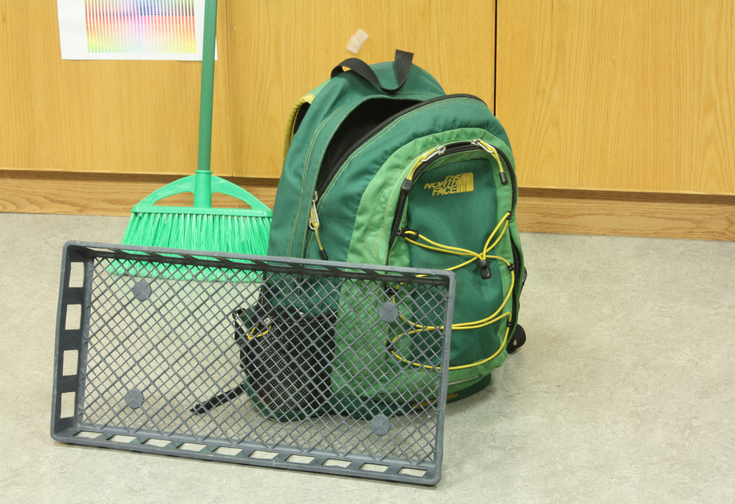
\includegraphics[scale=0.15]{./figures/im_left.png}
 		\caption{left image}
	\end{subfigure}
	\begin{subfigure}{0.49\linewidth}
		\centering
		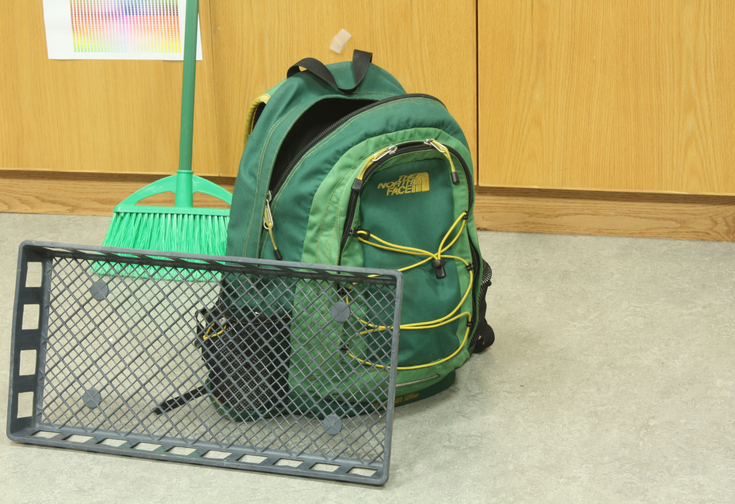
\includegraphics[scale=0.15]{./figures/im_right.png}
 		\caption{right image}
	\end{subfigure}
\caption{Given images for disparity map calculation}\label{fig:givenImages}
\end{figure}

\section{One thread implementation of ZNCC algorithm}\label{sec:CbasedImplementation}

The goal of the correspondence search is to find the corresponding pixel in the right image (a match) for the given pixel on the left image. Usually, comparing just pixels is not enough, therefore, their neighborhoods are compared.

In area based matching algorithms, rectangular blocks of pixels from a set of two images $W \times H$ (left and right images) are compared and matched. We conducted our experiments for the images presented in Fig.~\ref{fig:givenImages}. \fixit{ For each block of the right image, designated by reference window, a corresponding block in the left image is sought using a given similarity measure as main criteria. During the search process, the correspondent block of the left image is moved by integer increments $(c,l)$ around a predefined region, designated by \textit{search window}, and an array of similarity scores $d(c,l)$ is generated for integer disparity values. In this work, we suggest the size of searching and referenced windows is equal. The position $(c_m, l_m)$ of the moving block, corresponding to the maximum computed value of the considered similarity function $\otimes$ for that search window, is selected and chosen to compute the optimum disparity vector corresponding to that reference window. Hence, a matching dense field $\mathbf{D}(x,y)$ is obtained by using as many overlapping search windows as the number of pixels that compose the image, thus obtaining a single disparity vector for each pixel.

%which can be normalized by the means of the samples (images)

%Matching single pixels is nearly impossible, therefore every pixel is represented by a small region containing it, called correlation window. 
%The depth of an image pixel is the distance of the corresponding space point from the camera center. To estimate the depth map and detect 3D objects, the corresponding pixels in the left and right images have to be matched.


\begin{equation}
d(c,l) = \sum_{v=0}^{Rwidth}\sum_{u=0}^{Rlength}R\left(u,v\right)\otimes S\left(c+u,l+v\right)
\end{equation}

\begin{equation}
d(c_m,l_m) = argmax\{d(c,l): 0\leq c < S_w; 0\leq l < S_l \}
\end{equation}

\begin{equation}
\mathbf{D}(x,y) = \{ d_{xy}(c_m,l_m): 0\leq x < W; 0\leq l < H \}
\end{equation}

Many different similarity measures $\otimes$ have been referred in the literature. The reasons for a particular selection are usually related to the computational load, achieved performance and algorithmic simplicity. However, this work mostly concentrates on Zero-mean Normalized Cross-Correlation (ZNCC) similarity function:

\begin{equation}\label{eq:zncc}
ZNCC(R,S)=\frac{\left(R-\overline{R}\right) * \left(S-\overline{S}\right)}{\|R-\overline{R}\| \|S-\overline{S}\|}
\end{equation}
%$R\left(u,v\right)$
%$S\left(c,l\right)$

where numerator is the scalar product of the reference and search windows. $R$ denotes a reference window pixel, $S$ a search window pixel, $\overline{R}$ the local mean of the reference window: $\overline{R}=\sum_{v=0}^{Rlength}\sum_{u=0}^{Rwidth}R\left(u,v\right)$, and $\overline{S\left(c,l\right)}$ the pixel mean in the block of the search window being compared: $\overline{S\left(c,l\right)}=\sum_{v=0}^{Rlength}\sum_{u=0}^{Rwidth}S\left(c+u-d,l+v\right)$. The Euclidean norm is noted:
\begin{equation}
\|R\| = \sqrt{\sum_{v=0}^{Rlength}\sum_{u=0}^{Rwidth}\left(R\left(u,v\right) - \overline{R}\right)^2}
\end{equation}

Usually, the selection of the size of the reference window is not a simple and trivial task. It has been shown that the probability of a mismatch usually decreases as the size of the reference window increases. However, using large windows leads to an accuracy loss, since the influence of image differences increases greatly with the increase of the considered area. Therefore, this parameter must be great enough so that search window comprises the correspondent block of the given image. Furthermore, a difficult and important trade-off must be done when selecting this window size, since the computational load and processing time usually increase quadratically with the size of the window. Often, a compromise must be made, by adjusting these parameters according to the image size and contents. Taking into account all these factors and evaluating many experiments, we found that $3 \times 21$ is an optimal size of the window.

The estimation of dense disparity maps is usually performed by taking in consideration a set of constrains relating the two images being analyzed, making it possible to decrease the dimension and reduce the ambiguity of this problem, thus decreasing the total processing time. In this work, we admit two assumptions:
\begin{itemize}
	\item \textit{Epipolar Constrain:} allow to convert 2D search into 1D search. For the epipolar rectified image pair, each point in the left image lies on the same horizontal line (epipolar line) as in the right image. This approach is used to reduce a search space for depth map computation algorithms.
	\item \textit{Unicity:} imposes that each pixel can have, at most, one correspondent pixel in the other image.
\end{itemize}

\begin{figure}[t!]
\centering
	\begin{subfigure}{0.49\linewidth}
		\centering
		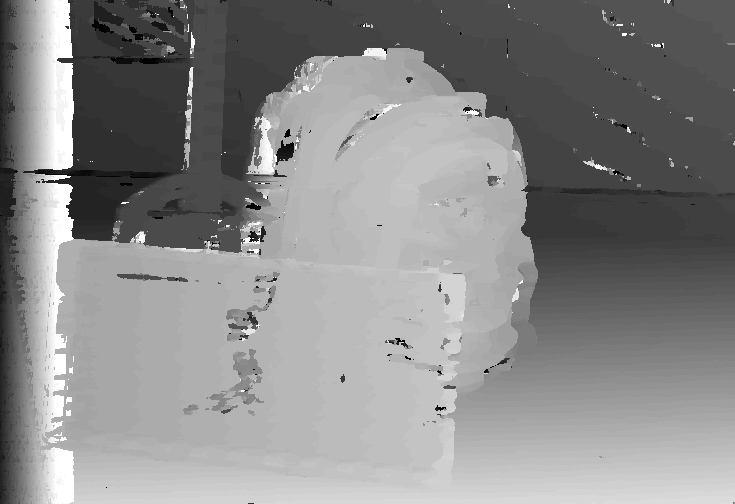
\includegraphics[scale=0.2]{./figures/left_dm.jpg}
 		\caption{Left disparity map}\label{subfig:leftDisparity}
	\end{subfigure}
	\begin{subfigure}{0.49\linewidth}
		\centering
		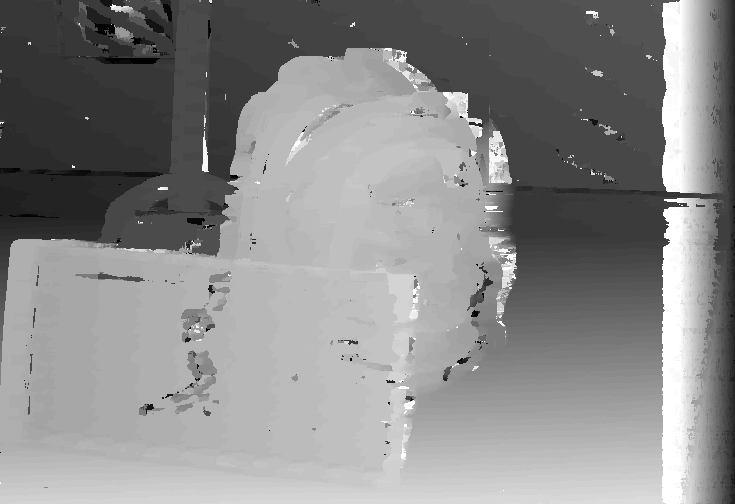
\includegraphics[scale=0.2]{./figures/right_dm.jpg}
 		\caption{Right disparity map}\label{subfig:rightDisparity}
	\end{subfigure}
\\
	\begin{subfigure}{\linewidth}
		\centering
		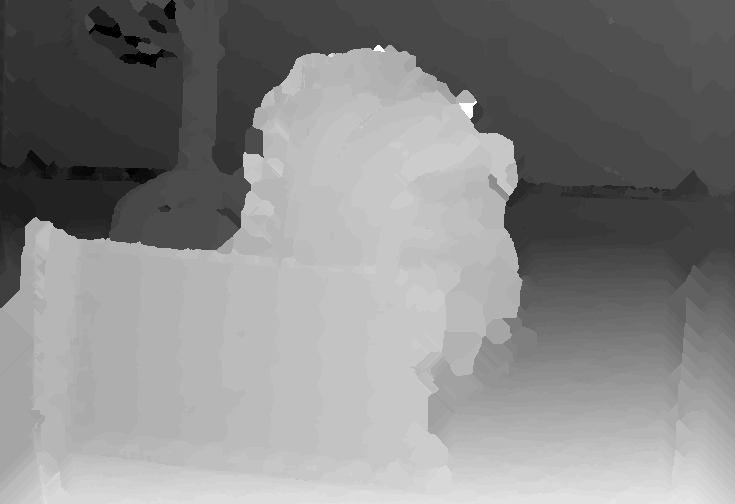
\includegraphics[scale=0.43]{./figures/final_dm.jpg}
 		\caption{The final disparity map}\label{subfig:finalDisparity}
	\end{subfigure}
\caption{Given images for disparity map calculation}\label{fig:disparities}
\end{figure}

Utilizing Eq.~\ref{eq:zncc}, we calculated disparity map for both images and for a disparity value \textit{d} from 0 to 64. The results are illustrated in Fig.~\ref{subfig:leftDisparity} and Fig.~\ref{subfig:rightDisparity} respectively. However, to compute Right-Left disparity we made a trick with setting up a disparity range. Specifically, the lower bound was initialized to -64 and the upper bound to 0. Computing the disparities is trivial: simply choose at each pixel the disparity associated with the minimum cost value. Thus, these methods perform a local 'winner-take-all' (WTA) optimization at each pixel. Once disparity map for both images was computed, we perform post-processing consisting of two stages: cross-checking and occlusion filling. Cross-checking is calculated by taking the computed disparity value in one image, and re-projecting it in the other image. If the difference in the values is higher than a given threshold (equals to 2 in our work), then the pixel value is initialized to 0. Occlusion filling was performed by applying the nearest neighbour interpolation. The final disparity map is illustrated in Fig.~\ref{subfig:finalDisparity}. It can clearly be seen that the proposed algorithm and post-processing steps allow to achieve good accuracy in calculation of disparity map. However, the computational load and elapsed time for this implementation are remarkably high. In following section, we propose an approach based on OpenCL technology which significantly improves performance.
}
\section{"Naive" OpenCL implementation}\label{sec:OpenclImplementation}
\subsection{Description}
In the so called "Naive implementation", we have not used any optimization recommended by manufacturers. We have created a 2-dimensional grid of work-groups of different sizes, where each work-item corresponded one pixel.

We have decided to create a separte kernel for each of the subproblems (resizing, zncc computation, cross-checking and occlusion filling): \textit{resize.cl}, \textit{zncc.cl}, \textit{cross\_check.cl} and \textit{occlusion.cl} respectively. We performed normalization of the disparity map on the CPU. The structure of the host code is presented in Algorithm \ref{hostcode}.


 \begin{algorithm}
 \caption{Host algorithm}\label{hostcode}
 \begin{algorithmic}[1]
 \renewcommand{\algorithmicrequire}{\textbf{Input:}}
 \renewcommand{\algorithmicensure}{\textbf{Output:}}
 \REQUIRE Images filenames.
  \STATE Check arguments.
  \STATE Read images.
  \STATE Chose the vendor and the device.
  \STATE Allocate memory on the device for the original images and the intermediate results.
  \STATE Copy the original images to the device, to the certain preallocated buffers.
  \STATE Consequently set arguments load kernels to the queue.
  \STATE Wait until the kernels execution is finished.
  \STATE Copy the result into host memory.
  \STATE Normalize the disparity map.
  \STATE Save the result to \textit{depthmap.png}.
 \end{algorithmic} 
 \end{algorithm}

The Naive implementation of the kernels does not utilize any local memory optimization tricks and basically uses two dimensional workers' identifiers instead of indicies of loops in the one thread implementation.

\section{Benchmarks}\label{sec:Benchmarks}
We have tested the Naive implementation on two different machines with Ubuntu 14.04 64 bit. Both machines have NVIDIA GPUs, the same version graphics drivers and CUDA 7.5. As a global size we took teh new image size -- $504\times735$. We enumerated all possible values of workgroup sizes using divisors of 504 and 735 and found out, that the work group size, which gives the best performance in our implementation of ZNCC is $3\times21$. We have also run our implementation on the laptop with Intel CPU 6200U skylake. However, OpenCL implementation turned out to be slower than the original C version. Most probably, it happened because of the communication overhead. We could improve the benchmark result, but decided to fucus only on GPU implementations. Our benchmark results (average of 3 launches) are presented in Table \ref{benchnaive}.
\begin{table}
\caption{Benchmarking of the naive OpenCL implementation}\label{benchnaive}
\centering
\begin{tabular}
{|c|C{1.5cm}|C{1.5cm}|C{1cm}|}
\hline
{\bfseries Device}  & {\bfseries Plain C time [sec]}  & {\bfseries GPU time [sec]} & {\bfseries Performance gain} \\
\hline
NVIDIA GTX960 OC & 84.9350 & 0.8356 & 101.65\\
\hline
NVIDIA GTX750 Titan & 77.5322 & 1.7745 & 43.7\\
\hline
\end{tabular}
\end{table}

In our testing equipment, the machine with the more powerful GPU had less powerful CPU than the machine with GTX750 (Intel(R) Core(TM) i5-3470 vs. Intel(R) Core(TM) i5-4570). By changing the processors, our performance gain would be still good -- 92.79. In this report, we consider it as our final result.

\section{Optimization of OpenCL kernels}\label{sec:Optimization}
\subsection{If-statements removal}
First kernel optimization which we have made was to remove extra if-statements in kernels which check the boundaries. The outcome of such modification was a slight performance improvement (improved value is presented in the Table \ref{benchnaive}).

\subsection{Local memory usage}
In our work we did not use any local memory tricks, but the potential usage of it would be in caching the blocks for the calculation of mean and standard deviation.

\section{Compiling and running}
We have tested our implementation on the following software: Ubuntu 14.04 64 bit, GCC compiler version 4.8.4, NVIDIA drivers 352.93, NVIDIA CUDA 7.5. In order to compile our code, the user just need to use make utility (see the Listing \ref{mylisting}).

\begin{lstlisting}[language=bash,caption={Compiling commands},label={mylisting}]
# Compile and run OpenCL code
make cl runcl
# Compile and run plain C code
make c runc
\end{lstlisting}

\section{Discussion and Conclusions}
In this work we have presented a Naive implementation of ZNCC algorithm using OpenCL. Despite of the fact, that We did not use any local memory tricks, we have shown, that it is possible to  achieve a quite good result of performance gain -- 92.79 on a machine with Intel(R) Core(TM) i5-4570 CPU @ 3.20GHz and GPU NVIDIA GTX960. We have also shown, that by changing the GPU to the newer generation, our performance gain has increased in more than twice.



\bibliographystyle{IEEEtran}
\bibliography{report}

\end{document}


